\mysubsectionformatted{Design Pattern Abstract Factory}
\myparagraph{
    \begin{tcolorbox}[colback=blue!5!white, colframe=blue!75!black]
        Il pattern permette di definire un'interfaccia astratta \textit{Factory} e
        altre classi \textbf{Factory} per ogni famiglia di elementi da creare.
        In questo modo, si possono creare delle famiglie di classi correlate tra loro
        che implementano un'interfaccia comune.
    \end{tcolorbox}

    \setcounter{figure}{0}
    \begin{figure}[h]
        \centering
        \caption{Esempio di Abstract Factory}
        \vspace{0.5cm}
        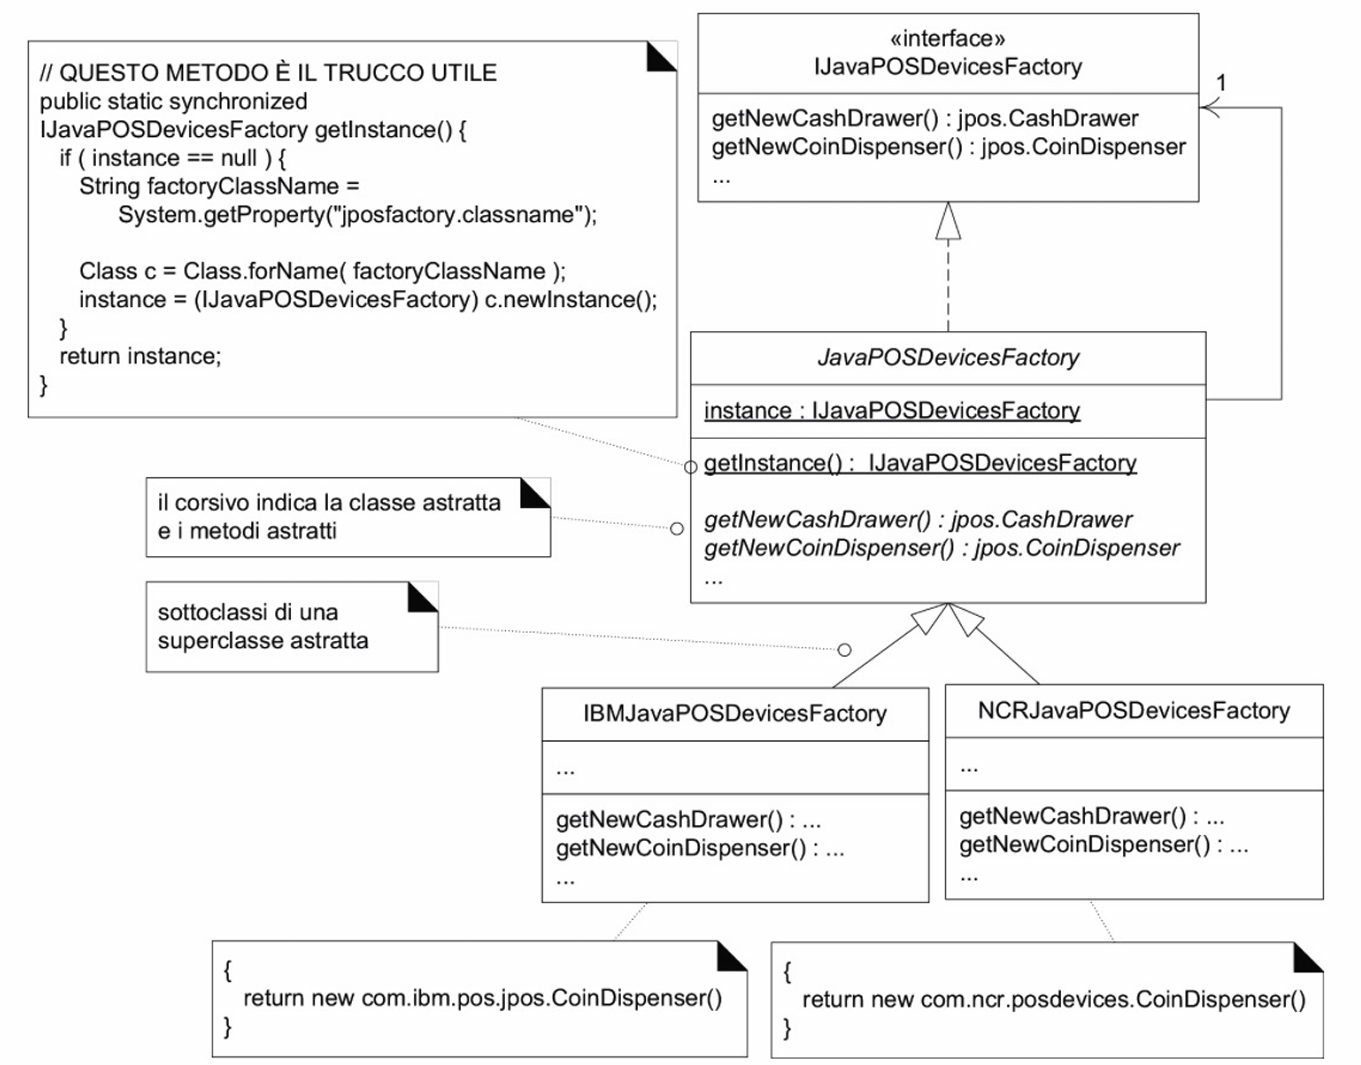
\includegraphics[scale=0.27]{Esercitazione - Design Patterns/Abstract Factory.png}
        \label{fig:pattern}
    \end{figure}

    Spesso, l'\textit{Abstract Factory} viene creata come \textbf{classe astratta}, non come \\interfaccia.\\
    La Factory legge dalle proprietà di sistema quale famiglia di oggetti creare, questo grazie all'aiuto
    del pattern \textbf{Singleton} (con il metodo \textit{getInstance()}).

    \newpage
    }
